\documentclass[11pt, a4paper]{article}

% --- Packages ---
\usepackage[
    ignoreheadfoot,
    top=1.5cm,      
    bottom=1.5cm,   
    left=1.5cm,     
    right=1.5cm,    
    footskip=0.8cm,
]{geometry}
\usepackage{titlesec}
\usepackage{enumitem}
\usepackage{fontawesome5}
\usepackage{xcolor}
\usepackage{graphicx}
\usepackage{hyperref}
\usepackage{needspace}

% --- Color Definitions ---
% Using a professional corporate blue
\definecolor{primaryColor}{RGB}{0, 79, 144}
\definecolor{darkGray}{RGB}{60, 60, 60}

% --- Hyperlinks ---
\hypersetup{
    colorlinks=true,
    urlcolor=primaryColor,
    linkcolor=primaryColor,
    pdfborder={0 0 0}
}

% --- Section Formatting ---
\titleformat{\section}
    {\large\bfseries\color{primaryColor}\uppercase}
    {}{0em}
    {}[\titlerule]
\titlespacing{\section}{0pt}{12pt}{8pt}

% --- List Formatting ---
\setlist[itemize]{
    leftmargin=*,
    label={\small\textbullet},
    nosep,
    topsep=4pt,
    itemsep=3pt
}

% --- Custom Commands ---
\newcommand{\entry}[4]{
    \textbf{#1} \hfill \textbf{#2} \\
    \textit{#3} \hfill \textit{#4}
}

\begin{document}

% --- HEADER (Dubai Standard) ---
\begin{center}
    \begin{minipage}[c]{0.72\textwidth}
        \raggedright
        {\Huge\textbf{\color{primaryColor}Razim Manzoor}} \\[6pt]
        \textbf{Business Analyst | AI Strategist | Automation Specialist} \\[4pt]
        
        \faMapMarker* \ Dubai, UAE \quad 
        \faPhone \ +971 50 300 1697 \quad 
        \faEnvelope \ \href{mailto:manzoorrazim@gmail.com}{manzoorrazim@gmail.com} \\
        \faLinkedin \ \href{https://www.linkedin.com/in/razim-manzoor}{linkedin.com/in/razim-manzoor} \\[8pt]
        
        % CRITICAL FOR DUBAI RECRUITMENT (Tier 2 Systems)
        \small 
        \textbf{Nationality:} Indian \quad | \quad \textbf{Visa Status:} Visit Visa (Available Immediately) \\
        \textbf{Date of Birth:} 25 May 2000 \quad | \quad \textbf{Marital Status:} Single
    \end{minipage}%
    \hfill
    \begin{minipage}[c]{0.25\textwidth}
        \raggedleft
        \IfFileExists{profpic.jpeg}{%
            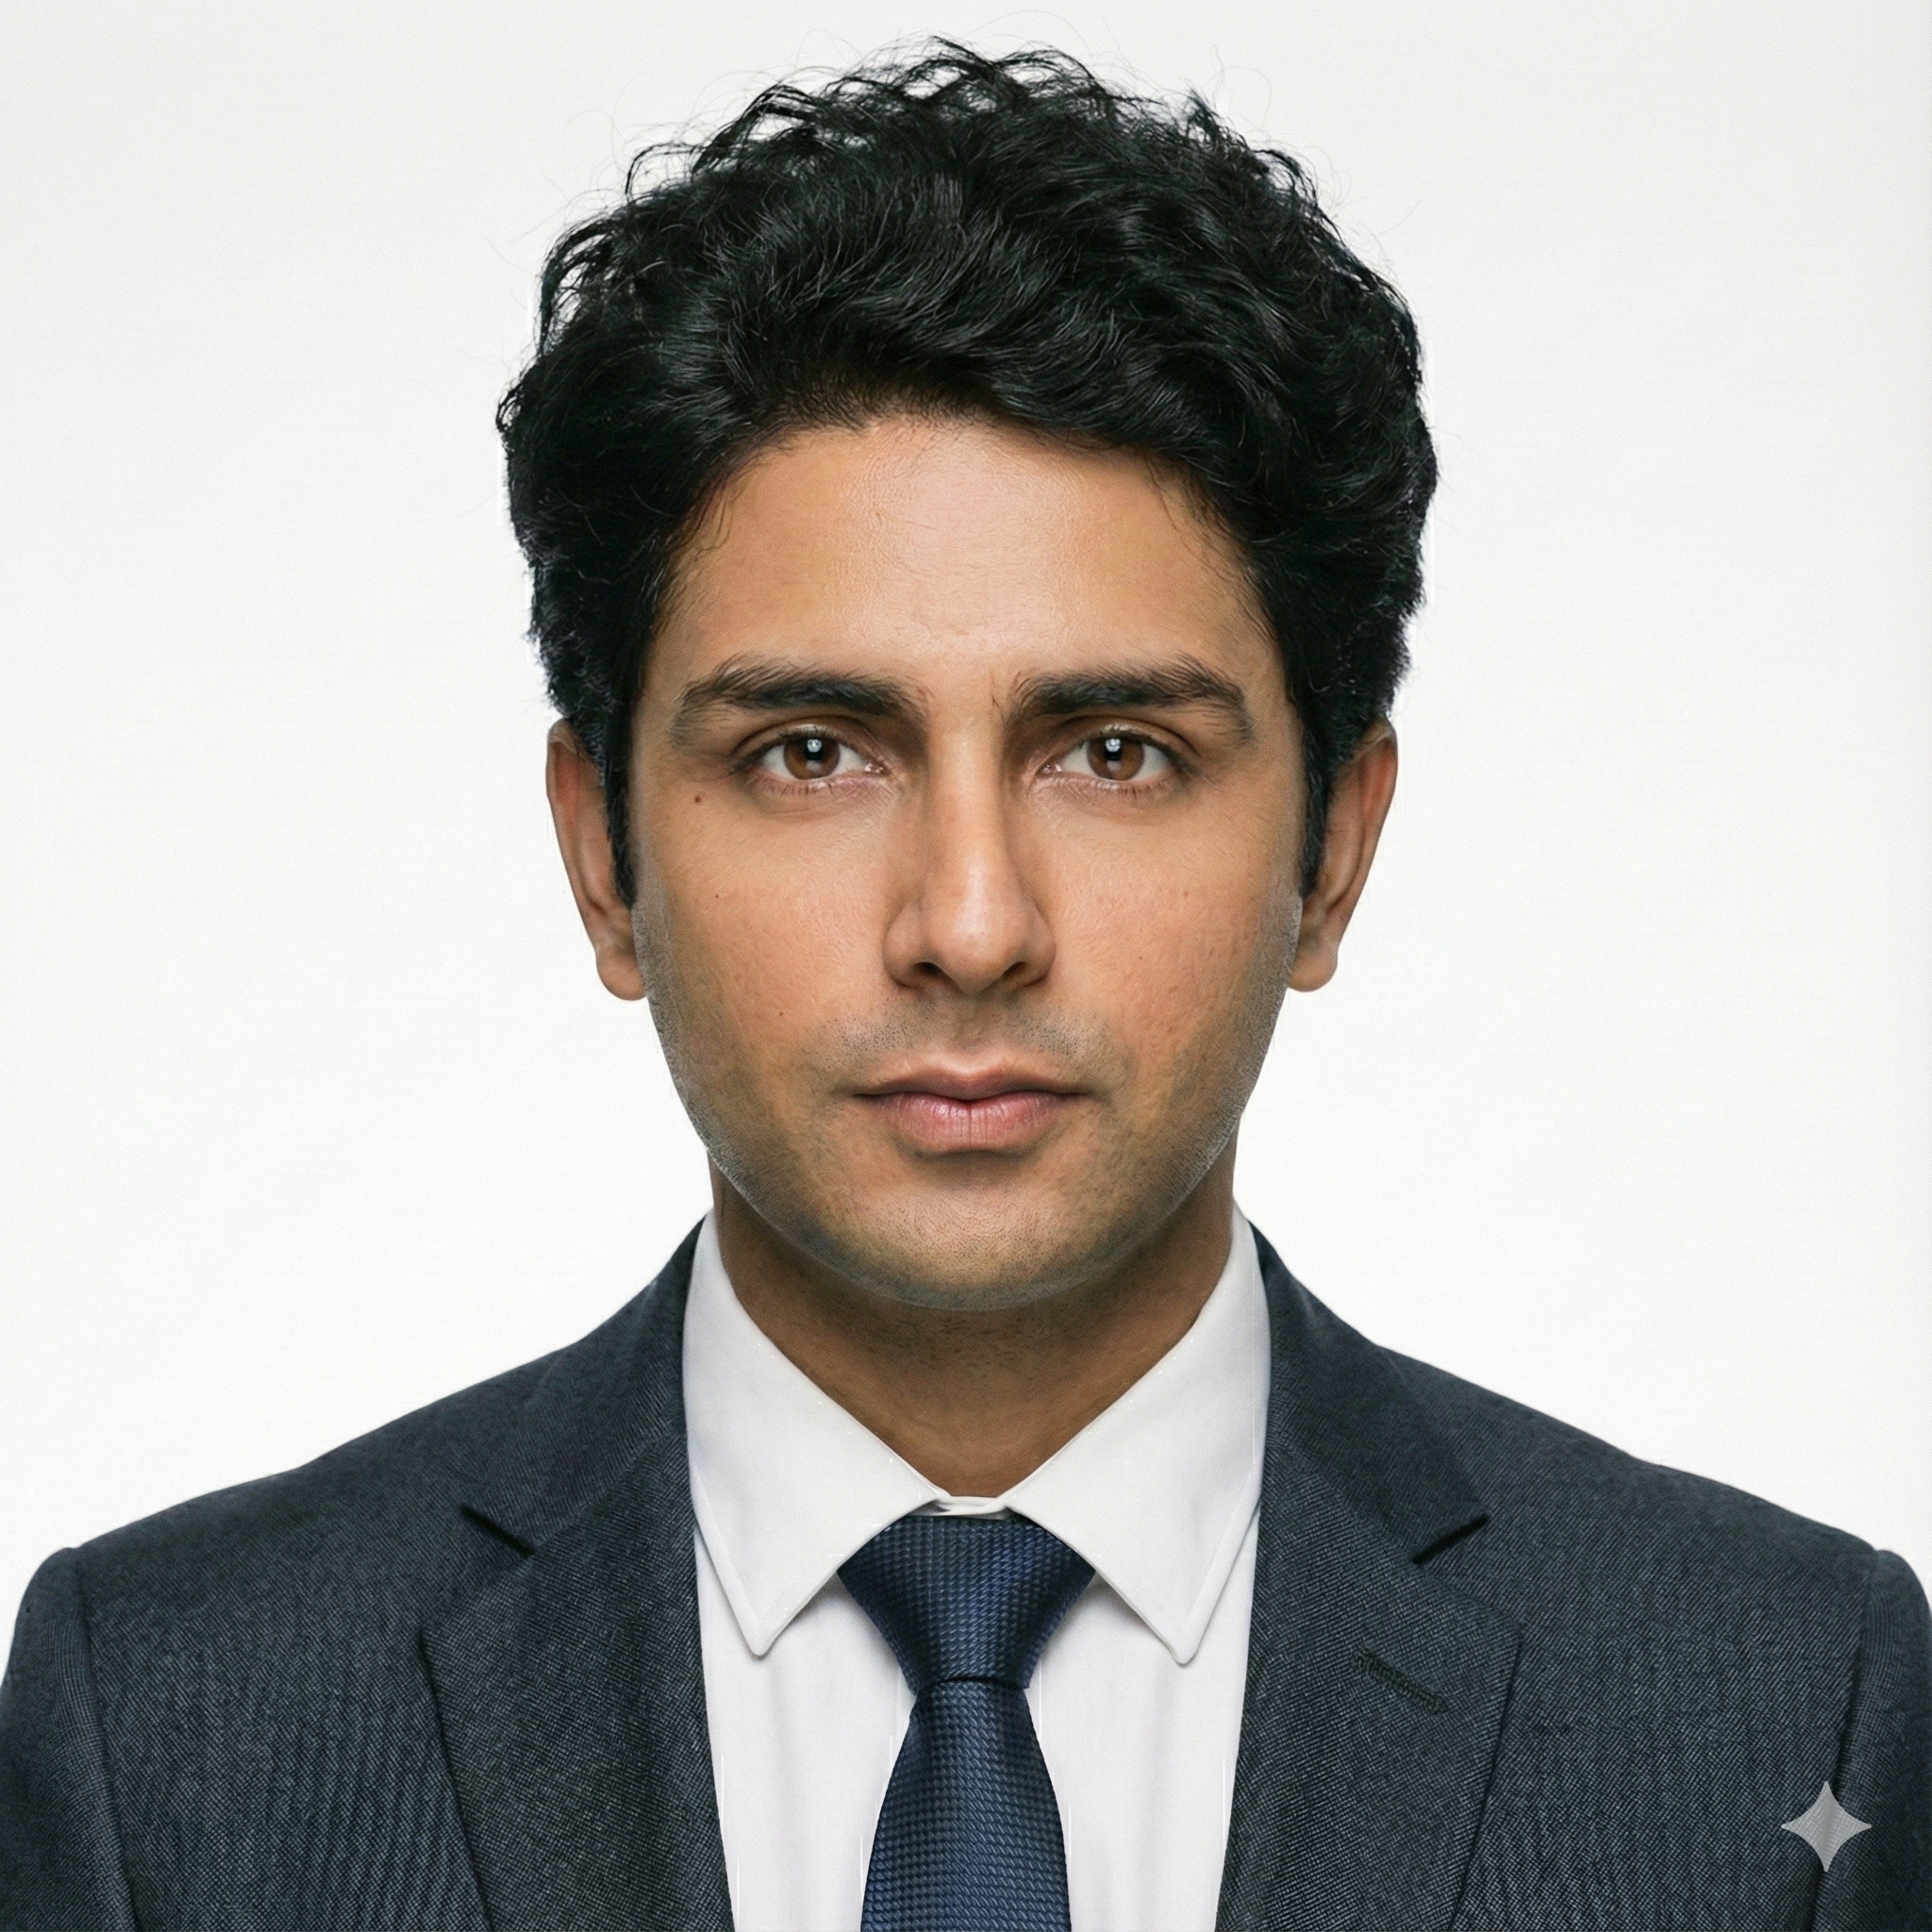
\includegraphics[width=3cm, keepaspectratio]{profpic.jpeg}%
        }{%
             \fcolorbox{gray}{white}{\parbox[c][3.5cm][c]{3cm}{\centering\tiny Photo Not Found\\(Name file profpic.jpeg)}}
        }%
    \end{minipage}
\end{center}

\vspace{0.2cm}

% --- PROFESSIONAL SUMMARY ---
\section{Professional Summary}
MBA-qualified Business Strategist and Data Analyst with a focus on \textbf{Digital Transformation} and \textbf{AI Implementation}. Proven ability to bridge the gap between technical data solutions and business goals. Expertise in building \textbf{Automated Workflows} (Power Automate), deploying \textbf{GenAI solutions} (RAG, LLMs) for operational efficiency, and creating real-time \textbf{BI Dashboards}. Specialized in translating complex data into actionable strategic insights to drive revenue growth and cost reduction.

% --- CORE COMPETENCIES ---
\section{Core Competencies \& AI Fluency}
\begin{itemize}[leftmargin=0pt, label={}]
    \item \textbf{Business Strategy:} Strategic Planning, KPI Analysis, Process Mining, ROI Assessment, Market Segmentation, Requirement Gathering, Stakeholder Management.
    \item \textbf{AI \& Automation:} Generative AI (LLMs), Retrieval-Augmented Generation (RAG), Prompt Engineering, AI Agents, Workflow Automation (Power Automate, UiPath).
    \item \textbf{Data Ecosystem:} Power BI (Advanced DAX), Python (Pandas, Scikit-learn), SQL, Azure, Tableau, Advanced Excel.
\end{itemize}

% --- PROFESSIONAL EXPERIENCE ---
\section{Professional Experience}

\entry{Data Science \& Business Intern}{Jun 2024 -- Apr 2025}{Luminar Technolab}{Kochi, India}
\begin{itemize}
    \item \textbf{Strategic Analysis:} Conducted market segmentation using statistical models to identify high-value customer clusters, revealing a \textbf{15\% revenue growth opportunity}.
    \item \textbf{Dashboard Development:} Accelerated executive decision-making by migrating manual reporting to real-time \textbf{Power BI dashboards}, reducing the reporting cycle from 3 days to 2 hours.
    \item \textbf{Customer Intelligence:} Applied \textbf{Sentiment Analysis} on unstructured customer feedback to guide product strategy for key SKUs, translating qualitative text into quantitative business metrics.
    \item \textbf{Data Integrity:} Performed extensive data cleansing and preparation to ensure the accuracy of analytical models and reports.
\end{itemize}

\vspace{8pt}

\entry{Associate AI and Data Analytics Engineer}{Nov 2023 -- May 2024}{Resemble Systems}{Kochi, India}
\begin{itemize}
    \item \textbf{Digital Transformation:} Led a finance automation initiative using \textbf{Power Automate}, streamlining invoice processing workflows which reduced manual data entry effort by \textbf{45\%}.
    \item \textbf{Process Optimization:} Conducted \textbf{Process Mining} to map operational workflows, identifying bottlenecks and implementing RPA solutions that improved cycle times by \textbf{20\%}.
    \item \textbf{Workforce Analytics:} Designed HR Analytics Dashboards to visualize attrition and engagement KPIs, enabling data-driven resource planning.
    \item \textbf{Cloud Integration:} Collaborated on deploying automated solutions via \textbf{Azure}, ensuring scalable and secure data handling.
\end{itemize}

% --- EDUCATION ---
\section{Education}
\entry{Master of Business Administration (MBA)}{2021 -- 2023}{JAIN University}{India}
\begin{itemize}
    \item \textit{Specialization:} Data Science \& Analytics
    \item \textit{Relevant Coursework:} Financial Analysis, Business Statistics, Marketing Analytics, Strategic Management.
\end{itemize}

\vspace{5pt}

\entry{Bachelor of Commerce (B.Com)}{2018 -- 2021}{Kannur University}{India}
\begin{itemize}
    \item \textit{Focus:} Computer Applications, Accounting Principles, Financial Management.
\end{itemize}

% --- PROJECTS ---
\section{Applied AI Projects}
\textbf{LiquidityAI: Automated Accounts Receivable Engine}
\begin{itemize}
    \item Developed a "Zero-Touch" Python system to automate invoice collections, reducing daily manual effort by \textbf{80\%} (3 hours to 5 minutes).
    \item Engineered a tiered logic gate (VIP vs. High Risk) to customize communication tone, preserving client relationships while optimizing liquidity recovery.
    \item Integrated a \textbf{Streamlit} dashboard with AI Agents for "Human-in-the-Loop" approval, ensuring contextual accuracy before dispatching emails.
\end{itemize}

\vspace{5pt}

\textbf{Secure Document Analysis Agent (Local RAG)}
\begin{itemize}
    \item Built a privacy-focused AI tool allowing businesses to query internal PDFs without external data exposure.
    \item Leveraged \textbf{DeepSeek \& Ollama} to create a local "Chat with your Data" solution, demonstrating cost-effective GenAI implementation for corporate knowledge management.
    \item Eliminated data leakage risks by ensuring 100\% offline processing, making the solution compliant with strict data handling protocols for sensitive documents.
\end{itemize}

\vspace{5pt}

\textbf{Automated Quality Control System (Computer Vision)}
\begin{itemize}
    \item Developed a \textbf{Convolutional Neural Network (CNN)} model to automate image classification, simulating an industrial Quality Assurance (QA) workflow.
    \item Applied data augmentation and preprocessing techniques to improve model robustness, ensuring consistent defect detection under varying conditions.
    \item Demonstrated the potential to significantly reduce manual inspection time and human error rates through automated visual validation.
\end{itemize}

% --- CERTIFICATIONS ---
\section{Certifications, Awards \& Virtual Experience}
\begin{itemize}
    % Combined section for maximum impact and efficient space usage
    \item \textbf{KPMG} -- Data Analytics Consulting Virtual Internship (Forage)
    \item \textbf{Accenture} -- Data Analytics \& Visualization Virtual Experience (Forage)
    \item \textbf{Google Advanced Data Analytics Professional Certificate} -- Coursera
    \item \textbf{Generative AI with Large Language Models} -- Coursera
    \item \textbf{Google Data Analytics Specialization} -- Coursera
    \item \textbf{1st Place}, Marketing Event -- Encore 2020 (South Indian Management Fest)
    \item \textbf{3rd Place}, Marketing Event -- Manaquest 2020 (National Level Management Fest)
\end{itemize}

% --- LANGUAGES ---
\section{Languages}
\begin{itemize}[leftmargin=0pt, label={}]
    \item \textbf{English:} Professional Working Proficiency
    \item \textbf{Malayalam:} Native / Bilingual Proficiency
    \item \textbf{Hindi:} Professional Working Proficiency
\end{itemize}

\end{document}